\documentclass{standalone}
\usepackage{tikz}
\usepackage{ctex,siunitx,bm}
\setCJKmainfont{Noto Serif CJK SC}
\usepackage{tkz-euclide,ninecolors}
\usepackage{amsmath}
\usetikzlibrary{patterns, calc}
\usetikzlibrary {decorations.pathmorphing, decorations.pathreplacing, decorations.shapes,}
\begin{document}
\small
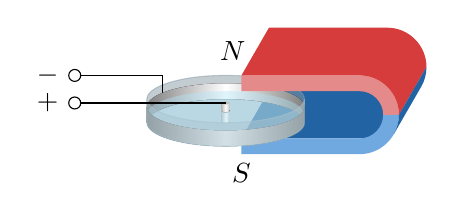
\begin{tikzpicture}[>=latex,scale=1.0]
  \fill[azure4](1.7,-0.4)--(0.2,-0.4)--++(60:0.7)--++(1.5,0)--++(0,-0.6);
  \fill[azure7](0.2,-0.4)--(1.7,-0.4)arc(-90:0:0.3)--++(0.2,0)arc(0:-90:0.5)--(0.2,-0.6)node[below,text=black]{$S$};
  \fill[cyan!30!gray,opacity=0.5](0,-0.2)ellipse(1 and 0.3);
  \fill[cyan!20!gray,opacity=0.5,draw,thin](-1,0.1)--(-1,-0.2)arc(180:0:1 and 0.3)--(1,0.1)arc(0:180:1 and 0.3);
  \draw[-o](-0.8,0)--++(0,0.4)--(-2,0.4)node[left]{$-$};
  \fill[left color= gray,right color=gray, middle color=white](-1,-0.2)arc(180:0:1 and 0.3)--(1,-0.2)--(1,0)arc(0:180:1 and 0.3)--cycle;
  \fill[left color= lightgray,right color=lightgray, middle color=white](-0.05,-0.2)rectangle(0.05,-0.05);
  \fill[cyan!30,opacity=0.4](0,-0.1)ellipse(1 and 0.3);
  \fill[left color= lightgray,right color=lightgray, middle color=white](0,-0.05)ellipse(0.05 and 0.02);
  \fill[left color= lightgray,right color=lightgray, middle color=white](-.05,-0.05)rectangle(0.05,0.05);
  \fill[lightgray](0,0.05)ellipse(0.05 and 0.02);
  \fill[left color= gray,right color=gray, middle color=white](-1,-0.2)arc(-180:0:1 and 0.3)--(1,-0.2)--(1,0)arc(0:-180:1 and 0.3)--cycle;
  \fill[cyan!20!lightgray,opacity=0.5,draw,thin](-1,0.1)--(-1,-0.2)arc(-180:0:1 and 0.3)--(1,0.1)arc(0:-180:1 and 0.3);
  \draw[-o](0,0.05)--(-2,0.05)node[left]{$+$};
  \fill[red7](2.0,-0.1)arc(0:90:0.3)--(0.2,0.2)--(0.2,0.4)--(1.7,0.4)arc(90:0:0.5)--cycle;
  \fill[red5](0.2,0.4)--++(60:0.7)node[midway,left,text=black]{$N$}--++(1.5,0)arc(90:0:0.5)--++(240:0.7)arc(0:90:0.5)--cycle;
  \fill[azure4](2.2,-0.1)arc(0:-30:0.5)--++(60:0.7)arc(-30:0:0.5)--cycle;
\end{tikzpicture}
\end{document}